\documentclass[12pt]{article}
%Paquetes
\usepackage[left=2cm,right=2cm,top=3cm,bottom=3cm,letterpaper]{geometry}
\usepackage{lmodern}
\usepackage[T1]{fontenc}
\usepackage[utf8]{inputenc}
\usepackage[spanish,activeacute]{babel}
\usepackage{mathtools}
\usepackage{amssymb}
\usepackage{enumerate}
\usepackage{tabularx}
\usepackage{wasysym}
\usepackage{listings}
\usepackage{graphicx}
\usepackage{hyperref}
\usepackage{graphicx}
\usepackage{multicol}
\usepackage{float}
\usepackage{booktabs}
\graphicspath { {media/} }
%\usepackage[document]{ragged2e}
% Package to generate and customize Algorithm as per ACM style
\usepackage[ruled]{algorithm2e}
\renewcommand{\algorithmcfname}{ALGORITHM}

% Preambulo
\title{Comparación entre el Algoritmo Genético Simple y el Algoritmo de Optimización Inspirado en Magnetismo con Repulsión de Corto Alcance aplicados al Problema del Agente Viajero}

\author{Andrea Itzel González Vargas \\
  Carlos Gerardo Acosta Hernández}
\date{Cómputo Evolutivo 2017-1 \\ Facultad de Ciencias UNAM \\ }
\begin{document}
\maketitle
\section{Introducción}
\subsection*{Panorama general}
Para este proyecto final decidimos realizar una comparación entre el Algoritmo Genético Simple (\textbf{AGS}) y el Algoritmo de Optimización Inspirado en Magnetismo (\textbf{MOA}),
con un operador enfocado a la \textbf{exploración}, propuesto en el artículo\footnote{Magnetic-inspired optimization algorithms: Operators and structures} que escogimos para la exposición en clase.

Como punto de referencia, elegimos implementar un programa similar al que hicimos primero para encontrar soluciones óptimas de
varias instancias del Problema del Agente Viajero (\textbf{TSP}) usando el MOA. Lo anterior por nuestra experiencia previa con el desarrollo del primer proyecto\footnote{Referencia al repositorio del primer proyecto}, que nos sirvió de guía para llevar a cabo la construcción de nuestra propia versión de un MOA aplicado a TSP.

La idea es verificar si el MOA, siendo una propuesta reciente\footnote{Propuesto por bla y bla} en el mundo del cómputo evolutivo, es una buena opción para resolver problemas de este tipo como ya hemos visto con el AGS y decidir si es en algún aspecto competitivo respecto a su adversario.
La entrada de ambos programas es una instancia del TSP, para la que ambos algoritmos mostrarán la mejor solución encontrada en cada una de sus iteraciones.

Para manejar y procesar las instancias del TSP, proporcionadas por la colección \textit{TSPLIB}\footnote{pagina oficial} y recopiladas en archivos individuales bajo el directorio \textit{tsp/}, hacemos uso de una
biblioteca para \textit{Java}, llamada \textit{TSPLIB4J}\footnote{referencia a su repo de github}.


\subsection*{Marco teórico}
Creemos que ya no es necesario ser muy específicos respecto al AGS implementado y presentado previamente en nuestro primer proyecto, por lo que esta
sección referirá únicamente al MOA.\\

En la teoría de los campos magnéticos, las partículas pueden atraerse o repelerse unas con otras dependiendo de su polaridad.
Como muchos algoritmos en el campo de estudio de la optimización, el MOA es una propuesta inspirada en este principio observado en la naturaleza.
Para este algoritmo, el conjunto de posibles soluciones son partículas con propiedades magnéticas, diseminadas en el espacio de búsqueda, donde cada
partícula es capaz de incidir una sobre la otra con una fuerza de atracción de largo alcance -tal como el concepto de fuerza electromagnética.

Similar a los algoritmos de optimización por enjambre o nube de partículas (\textbf{PSO}\footnote{En inglés: Particle Swarm Optimization}), donde
los individuos buscan imitar a aquel con mayor grado de adaptación, las partículas en el MOA con mejor calificación poseen masa y campo
magnético mayores, resultando en una mayor fuerza de atracción ejercida sobre las otras partículas.

Por un lado, este comportamiento cubre el concepto de explotación revisado en nuestro curso, sin embargo, el MOA cuenta además con una mejora
considerable respecto a los PSO convencionales.

Es considerado una de las debilidades de los PSO, el hecho de que sólo las mejores partículas, son las que
tienen una repercusión significativa sobre las demás menos adaptadas, que no tienen incidencia en otras.
En este sentido, estos algoritmos dejan fuera de consideración, importante información que pueden contener las partículas con bajo grado de
adaptación. Es por ello que en el esquema del MOA que revisamos, se considera la posibilidad de que todos las partículas cuenten con cierto
potencial de atracción, independientemente de su grado de adaptación (aunque éste lo afecte en magnitud).

Asimísmo, se incluye un operador de repulsión de corto alcance (\textbf{SRR}\footnote{En inglés: Short-Range Repulsion}). Este operador -que explicaremos más ampliamente en secciones posteriores-, permite que el algoritmo no se concentre únicamente en las partículas más cercanas a la solución, pues actúa como a manera de repulsión cuando la distancia entre dos partículas es menor a cierto umbral predefinido, manteniendo la diversidad y previniendo una convergencia prematura en óptimos locales.

Además del esfuerzo implementado para la optimización de ``tours'' en las instancias del TSP, el MOA ya ha sido puesto a prueba en varias aplicaciones de Inteligencia Artificial, como el entrenamiento de redes neuronales y ha sido propuesta ya una versión binaria del algoritmo.
Las implementaciones de los MOA, resultan en un paradigma dual de interacción entre partículas con la fuerza de repulsión/atracción, que puede
devenir un balance entre exploración y explotación.

Siguiendo esa línea, las virtudes que supone el esquema del MOA parecen prometedoras frente a la contraparte de este proyecto, el AGS.

\newpage
\subsection*{Herramientas}
Como herramienta fundamental, proporcionamos el pseudo-código del MOA básico que no contempla más operadores que el de actualización de posición de una partícula dada su velocidad.\\



\label{alg:moa}
  \begin{algorithm}[H]
    % \SetAlgoNoLine
%\KwIn{Archivo con instancia del Problema del Agente Viajero de TSPLIB}
%\KwOut{Mejor partícula por generación}
$t \gets 0$;
$X^t \gets randomValidPopulation$()\;
\Repeat{t = maxGen}{
  $t \gets t+1$\;
  \For{each $x$ in $X^t$}
  {
   evaluate $x$ and store performance in magnetic fields $B^t$;    
  }
  {
    Normalize  $B^t$\;
    \For{each $x$ in $X^t$}{
      evaluate mass of $x$ and store it in $M^t$\;
    }
    \For{all $x_{ij}^{t}$ in $X^t$}{
      $F_{ij} \gets 0$\;
      find $Nij$\;
      \For{each $x_{uv}^{t}$ in $N_{ij}$}{
        $F_{ij} \gets F_{ij} +  \displaystyle{(x_{uv}^t-x_{ij}^t)\times B^t \over D(x_{ij}^t,x_{uv}^t)}$;
      }
    }
    \For{all $x_{ij}^t$ in $X^t$}{
      $v_{ij,k}^{t+1}$ = $\displaystyle{F_{ij,k} \over M_{ij,k}} \times R(u_k,l_k)$\;
      $x_{ij,k}^{t+1}$ = $x_{ij,k}^{t} + v_{ij,k}^{t+1}$\;
    }
  }
}

\caption{Magnetic-inspired Optimization Algorithm (MOA)}
\end{algorithm}
\noindent
$N_{ij}$ := Conjunto de vecinos de la partícula $x_{ij}$.\\
$F_{ij}$ := Fuerza de atracción ejercida sobre la partícula $x_{ij}$.\\
$D(x_1,x_2)$ := Distancia entre $x_1$ y $x_2$.\\

\subsection*{Esquema}
Las figuras siguientes refieren a dos elementos más del esquema de
implementación que consideramos relevantes destacar: El operador de repulsión y la forma de la estructura de la población del MOA.\newpage
\begin{multicols}{2}
\begin{figure}[H]
  \centering
  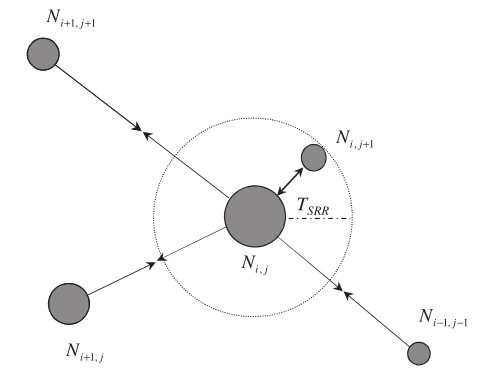
\includegraphics[width=.5\textwidth]{SRR}
  \caption{Representación del umbral $T_{SRR}$ de acción del operador SRR.}
\end{figure}
\begin{figure}[H]
  \centering
  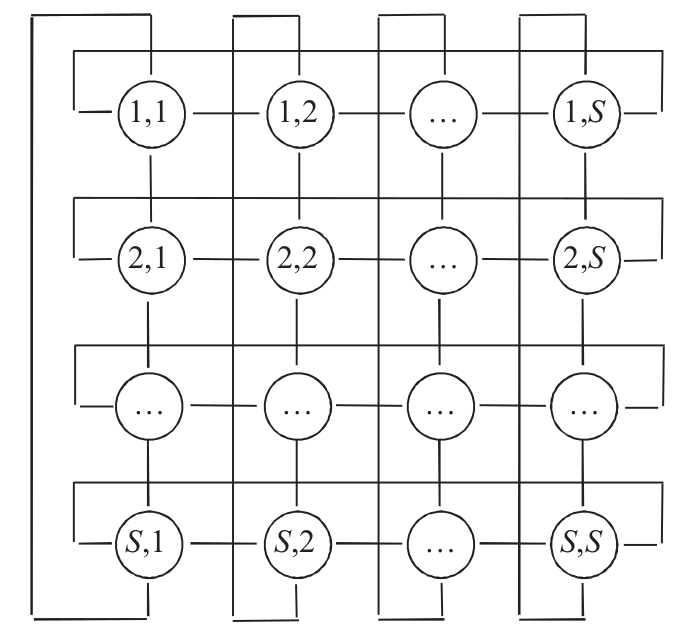
\includegraphics[width=.437\textwidth]{cell}
  \caption{Estructura de la población. Cada nodo es una partícula.}
\end{figure}
\end{multicols}

\subsection*{Datos de la computadoraexperimental}
ajsnjfjdfj

\subsection*{Diseño de implementación}
aqui decimos cosas de que lo hicimos todo nos y maldecimos a ismail
y a los 8 ñericks.

Más detalles sobre el diseño de la implementación se pueden encontrar en la Sección \ref{sec:esp} y siempre se puede consultar el código fuente
del proyecto en el directorio \textit{src/}.\\

A partir de ahora, nos referiremos a la implementación del MOA como SRMOA, por el operador que incluye en su ejecución.
\newpage
\section{Planteamiento}
\subsection*{Objetivo}
Determinar si el SRMOA (Tipo III) es una opción cuyo desempeño es competente respecto al algoritmo genético simple (AGS) en la resolución del problema del agente viajero (TSP).
\subsection*{Hipótesis}
 Esperamos que ambos tengan un desempeño similar para las distintas instancias del TSP. Creemos también que conforme la dimensión de las instancias del TSP crezcan, el SRMOA tendrá una mejora significativa respecto a instancias menores y pueda superar al AGS en tales magnitudes.  Respaldando ésta hipótesis tenemos las conclusiones del artículo sobre el MOA que mostraba que mientras mas crecía el problema, el SRMOA mejoraba su desempeño. Mientras que por otro lado nuestras pruebas con el AGS nos hacían ver que mientras más crecía el problema, disminuía el desempeño de éste algoritmo.

Asimismo, suponemos que la implementación del SRMOA será más sencilla que la del AGS.
\subsection*{Metodología}\label{sec:met}
Implementaremos el SRMOA y utilizaremos el AGS que previamente implementamos para el Proyecto 1. Probaremos los algoritmos con los archivos \textit{burma14}, \textit{ulysses16},\textit{gr17}, \textit{kroA100} y \textit{pr264}. Para cada archivo las tuplas de parámetros de las tablas siguientes un total de cinco veces. En conjunto se harán 25 corridas por algoritmo.\\


Los \textbf{parámetros} que se utilizarán para el \textbf{AGS} serán:
\begin{center}
\begin{tabularx}{0.25\textwidth}{|X|X|}
  \hline
\textbf{Pc} &  \textbf{Pm} \\ \hline
0.6 & 0.001 \\ \hline
\end{tabularx}
\end{center}

Y para el \textbf{SRMOA}:
\begin{center}
\begin{tabularx}{0.30\textwidth}{|X|X|X|X|}
  \hline
\textbf{$\alpha$} &  \textbf{$\rho$} & \textbf{$T_{SRR}$} & \textbf{$C_{SRR}$}\\ \hline
100 & 100 & 1 & 0.1 \\ \hline
\end{tabularx}
\end{center}

Para ambos algoritmos, se fijará el tamaño de la \textbf{población} en 225 individuos y se establecerá 1000 como máximo número de \textbf{generaciones} (siendo este el criterio de detención de las iteraciones).

Para hacer la comparación entre ambos algoritmos graficaremos el exceso porcentual promedio de peso del mejor circuito vs el número de generaciones de cada archivo para cada algoritmo, a demás del promedio del conjunto de los cinco archivos. Compararemos también el tiempo promedio que se tardó cada algoritmo para correr cada archivo.

\newpage

\section{Especificación}\label{sec:esp}
Esta sección cubre los aspectos más relevantes del diseño y construcción
de nuestro SRMOA. Si en algún momento de la lectura llega a ser confuso
de qué paso o etapa del algoritmo estamos elaborando, recomendamos volver a revisar el pseudocódigo del algoritmo básico (\ref{alg:moa} MOA).
\subsubsection*{Codificación del problema}
La codificación del problema se realizó de manera similar a la codificación del AGS implementado en el primer proyecto de la materia, puesto que
cada individuo contaba tanto en su fenotipo como en su genotipo, una permutación de las ciudades sin repeticiones de la instancia del TSP; el arreglo asociado, representa la ruta propuesta por el individuo.

En este caso, se trata de partículas con una ruta asociada, un vector de ciudades que determinan la posición de dicha partícula en el espacio de
búsqueda y que será alterada dependendiendo de la velocidad calculada por el cociente de la fuerza de atracción ejercida por sus vecinos y su masa,
junto con un factor aleatorio (\ref{sec:vel}).

Por ejemplo, para una partícula $x$ con posición $i,j$ en la estructura celular en la generación $t$,
$x_{ij}^t = [1,3,2,4,5]$, la ruta propuesta sería: $C_1 \to C_3 \to C_2 \to C_4 \to C_5 \to C_1$, $C_i \in P$, considerando a $P$ el conjunto de ciudades de la instancia de TSP.

Con el fin de evitar la implementación de un corrector de partículas, la generación de la población inicial aleatoria, se realizó con cuidado de asignar cada ciudad elegida aleatoriamente de $P$ sólo una vez por individuo. Acorde a esa intención, el operador velocidad que afecta la posición de una partícula, i.e. su ruta, realiza permutaciones entre las ciudades de dicha partícula únicamente, por lo que no existe el riesgo de invalidar una propuesta de ``tour'' al aplicarlo.

\subsubsection*{Evaluación de la población}
La evaluación de la población en un primer momento se realiza calculando el costo de la ruta propuesta por cada partícula. Tratando de seguir un
desarrollo similar al que experimentamos con el AGS en el primer proyecto, efectuamos el cálculo del costo de la siguiente manera:
\begin{equation}
  Costo(x) = d(x[0],x[n-1]) + \sum\limits_{i=0}^{n-2} d(x[i],x[i+1])
\end{equation}
Donde $x[i]$ corresponde a una de las ciudades representadas por la posición de la partícula $x$, y $n$ es la dimensión del espacio de búsqueda (el total de ciudades de la instancia del TSP).

Una vez obtenido el costo de todos los viajes -como vimos en el proyecto
anterior, no es posible utilizar este valor como ``fitness'' para nuestro algoritmo de optimización, pues el objetivo es minimizar ese costo-,
tal como en el AGS, decidimos considerar la función de
adaptación como sigue:
\begin{equation}
  fun(x) = (Costo_{max} + Costo_{min})-Costo(x)
\end{equation}
Al término el cálculo del desempeño de cada partícula, se almacena en uno de los atributos de la partícula, que corresponde a su campo magnético.

\subsubsection*{Campos magnéticos}
\subsubsection*{Masa}
\subsubsection*{Fuerza de atracción}

\subsection*{Operadores}
\subsubsection*{Velocidad}\label{sec:vel}

\subsubsection*{SRR}
\newpage
\section{Experimentación}
Con los parámetros determinados en la sección del planteamiento del
proyecto (\ref{sec:met} \textit{Metodología}), en esta sección incluímos las siguientes gráficas, una por cada instancia del TSP que elegimos, para representar visualmente el exceso porcentual promedio respecto de las generaciones del total de ejecuciones realizadas sobre cada archivo.
Para hacer aún más sencilla la observación comparativa, están representados con acotaciones de color ambos algoritmos.

\subsection{Instancia burma14}
\begin{figure}[H]
  \centering
  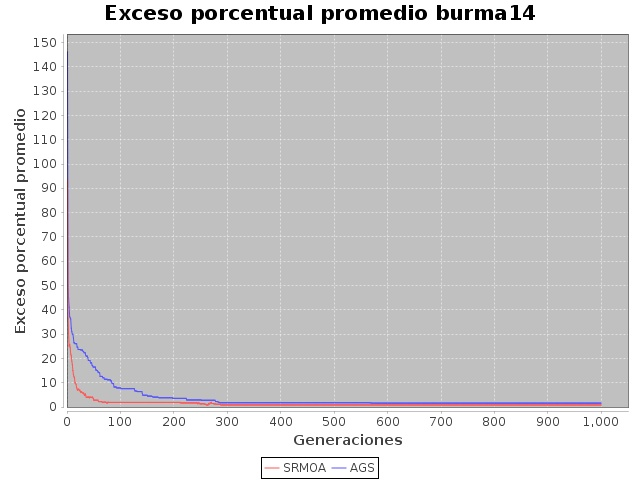
\includegraphics[width=1\textwidth]{graficas/burma14}
  \caption{Exceso porcentual promedio por generación en instancia de TSP con 14 ciudades.}
\end{figure}
\subsection{Instancia ulysses16}
\begin{figure}[H]
  \centering
  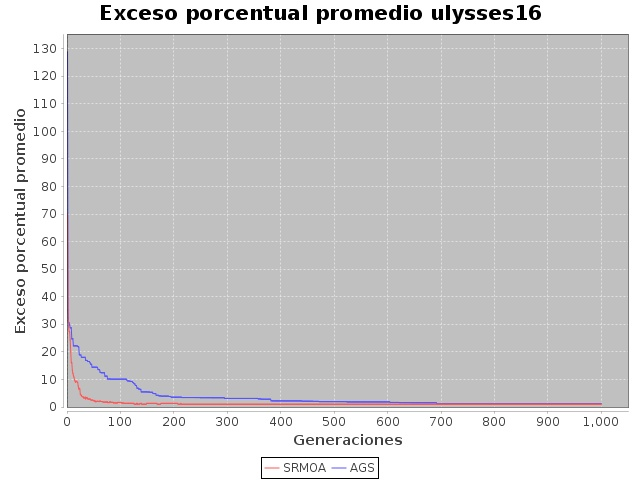
\includegraphics[width=1\textwidth]{graficas/ulysses16}
  \caption{Exceso porcentual promedio por generación en instancia de TSP con 16 ciudades.}
\end{figure}
\subsection{Instancia gr17}
\begin{figure}[H]
  \centering
  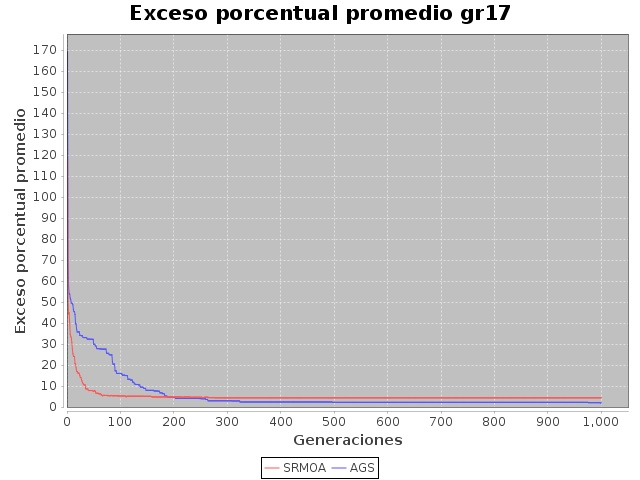
\includegraphics[width=1\textwidth]{graficas/gr17}
  \caption{Exceso porcentual promedio por generación en instancia de TSP con 17 ciudades.}
\end{figure}
\subsection{Instancia kroA100}
\begin{figure}[H]
  \centering
  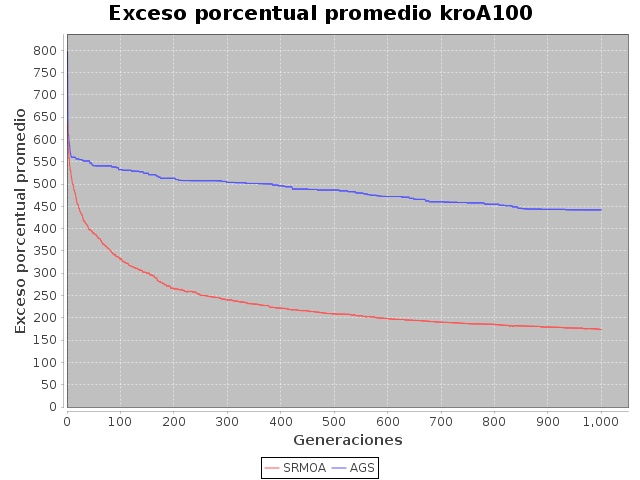
\includegraphics[width=1\textwidth]{graficas/kroA100}
  \caption{Exceso porcentual promedio por generación en instancia de TSP con 100 ciudades.}
\end{figure}
\subsection{Instancia pr264}
\begin{figure}[H]
  \centering
  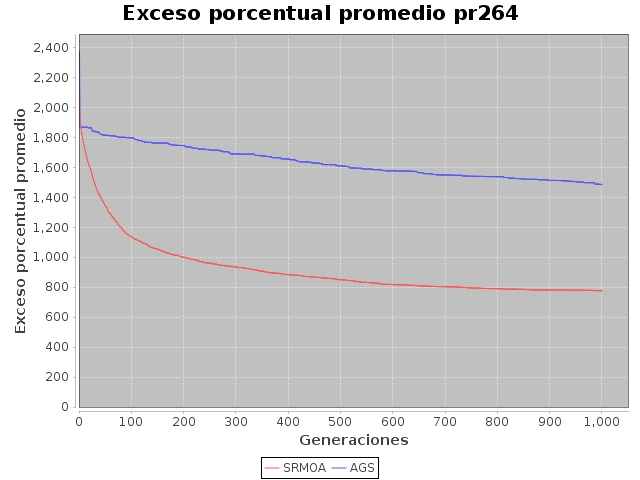
\includegraphics[width=1\textwidth]{graficas/pr264}
  \caption{Exceso porcentual promedio por generación en instancia de TSP con 264 ciudades.}
\end{figure}
\subsection{Total}
\begin{figure}[H]
  \centering
  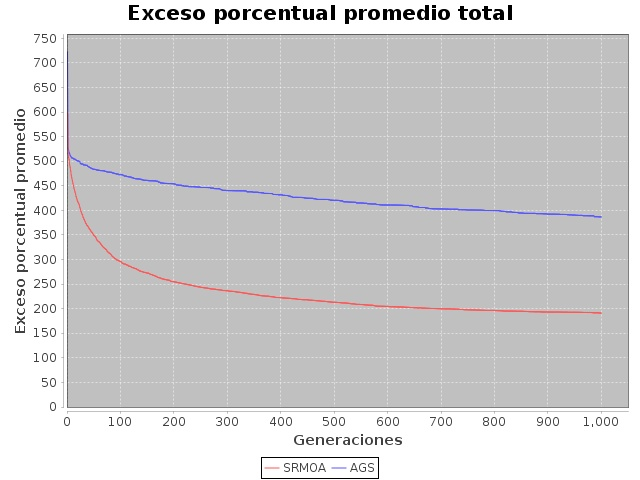
\includegraphics[width=1\textwidth]{graficas/total}
  \caption{Exceso porcentual promedio por generación para todas las instancias de TSP escogidas (burma14, ulysses16, gr17, kroA100, pr264).}
\end{figure}

\newpage
\subsection{Tiempo de ejecución}
Con el fin de ser más específicos respecto de la representación visual
previa de la experimentación que se llevó a cabo, proporcionamos los siguientes cuadros de datos. En conjunto, forman una tabla completa de valores de exceso porcentual y tiempo de ejecución por generación en el procesamiento de cada instancia del TSP. Se contemplan en el primer cuadro, \textit{burma14}, \textit{ulysses16}, \textit{gr17}, \textit{kroA100}, \textit{pr264}.

\begin{table}[H]
  \centering
  \caption{Exceso porcentual promedio y tiempo de ejecución por generación}
  \scalebox{0.6}{
    \begin{tabular}{ |c |c | c | c | c | c | c | c | c | c | c | c | c | }
      \hline
      Generación
      & \multicolumn{4}{c|}{burma14}
      & \multicolumn{4}{c|}{ulysses16}
      & \multicolumn{4}{c|}{gr17} \\\cline{2-13}
      & \multicolumn{2}{c|}{SRMOA} & \multicolumn{2}{c|}{AGS}
      & \multicolumn{2}{c|}{SRMOA} & \multicolumn{2}{c|}{AGS}
      & \multicolumn{2}{c|}{SRMOA} & \multicolumn{2}{c|}{AGS} \\\cline{2-13}
      & Exceso $\%$  & Tiempo (s) & Exceso $\%$  & Tiempo (s) 
      & Exceso $\%$  & Tiempo (s) & Exceso $\%$  & Tiempo (s) 
      & Exceso $\%$  & Tiempo (s) & Exceso $\%$  & Tiempo (s)   \\ \hline
      1
      & 93.50 & 0.0034 & 146.19 & 0.0182
      & 69.89 & 0.0032 & 128.91 & 0.0032
      & 117.99 & 0.0010 & 169.26 & 0.0010 \\ \hline
      50
      & 2.82 & 0.3458 & 16.46 & 0.2032
      & 2.38 & 0.3842 & 14.44 & 0.2098
      & 7.54 & 0.0838 & 29.88 & 0.1044 \\ \hline
      100
      & 1.88 & 0.6656 & 7.85 & 0.3990
      & 1.58 & 0.7614 & 10.09 & 0.4278
      & 5.28 & 0.1656 & 15.99 & 0.1944 \\ \hline
      150
      & 1.88 & 0.9826 & 4.83 & 0.6004
      & 1.31 & 1.1378 & 5.45 & 0.6168
      & 5.10 & 0.2474 & 7.93 & 0.2876 \\ \hline
      200
      & 1.88 & 1.3000 & 3.54 & 0.8102
      & 1.31 & 1.5136 & 3.55 & 0.8178
      & 4.79 & 0.3290 & 4.52 & 0.3798 \\ \hline
      250
      & 1.39 & 1.6190 & 2.90 & 0.9868
      & 0.99 & 1.8904 & 3.39 & 1.0036
      & 4.66 & 0.4106 & 4.03 & 0.4652 \\ \hline
      300
      & 0.85 & 1.9368 & 1.76 & 1.1594
      & 0.99 & 2.2666 & 3.10 & 1.2038
      & 4.36 & 0.4936 & 2.96 & 0.5478 \\ \hline
      350
      & 0.85 & 2.2546 & 1.76 & 1.3646
      & 0.99 & 2.6424 & 3.10 & 1.3970
      & 4.36 & 0.5746 & 2.38 & 0.6684 \\ \hline
      400
      & 0.85 & 2.5712 & 1.76 & 1.5266
      & 0.99 & 3.0182 & 2.22 & 1.5856
      & 4.36 & 0.6658 & 2.38 & 0.7786 \\ \hline
      450
      & 0.85 & 2.8880 & 1.76 & 1.6884
      & 0.99 & 3.3940 & 2.09 & 1.7700
      & 4.36 & 0.7538 & 2.38 & 0.8808 \\ \hline
      500
      & 0.85 & 3.2046 & 1.76 & 1.8606
      & 0.99 & 3.7878 & 1.95 & 1.9508
      & 4.36 & 0.8354 & 2.22 & 0.9812 \\ \hline
      550
      & 0.85 & 3.5212 & 1.76 & 2.0224
      & 0.99 & 4.1638 & 1.85 & 2.1316
      & 4.36 & 0.9170 & 2.22 & 1.0768 \\ \hline
      600
      & 0.85 & 3.8378 & 1.59 & 2.1810
      & 0.99 & 4.5392 & 1.85 & 2.3140
      & 4.36 & 0.9980 & 2.22 & 1.1714 \\ \hline
      650
      & 0.85 & 4.1548 & 1.59 & 2.3378
      & 0.99 & 4.9330 & 1.55 & 2.5072
      & 4.36 & 1.0790 & 2.22 & 1.2732 \\ \hline
      700
      & 0.85 & 4.4710 & 1.59 & 2.5034
      & 0.99 & 5.3084 & 1.23 & 2.6960
      & 4.36 & 1.1596 & 2.22 & 1.3606 \\ \hline
      750
      & 0.85 & 4.7882 & 1.59 & 2.6880
      & 0.99 & 5.6840 & 1.23 & 2.9016
      & 4.36 & 1.2412 & 2.22 & 1.4518 \\ \hline
      800
      & 0.85 & 5.1052 & 1.59 & 2.8474
      & 0.99 & 6.0600 & 1.23 & 3.1092
      & 4.36 & 1.3228 & 2.22 & 1.5438 \\ \hline
      850
      & 0.85 & 5.4226 & 1.59 & 3.0052
      & 0.99 & 6.4356 & 1.23 & 3.3062
      & 4.36 & 1.4040 & 2.22 & 1.6290 \\ \hline
      900
      & 0.85 & 5.7474 & 1.59 & 3.1816
      & 0.99 & 6.8112 & 1.23 & 3.5036
      & 4.36 & 1.4872 & 2.22 & 1.7130 \\ \hline
      950
      & 0.85 & 6.0736 & 1.59 & 3.3486
      & 0.99 & 7.1868 & 1.23 & 3.7024
      & 4.36 & 1.5696 & 2.22 & 1.8182 \\ \hline
      1000
      & 0.85 & 6.3904 & 1.59 & 3.5432
      & 0.99 & 7.5624 & 1.23 & 3.8978
      & 4.36 & 1.6516 & 1.96 & 1.9106 \\ \hline
    \end{tabular}
  }
\end{table}

\begin{table}[ht]
  \centering
  \caption{Exceso porcentual promedio y tiempo de ejecución por generación}
  \scalebox{0.6}{
    \begin{tabular}{ |c |c | c | c | c | c | c | c | c | c | c | c | c | }
      \hline
      Generación
      & \multicolumn{4}{c|}{kroA100}
      & \multicolumn{4}{c|}{pr264}
      & \multicolumn{4}{c|}{Total} \\\cline{2-13}
      & \multicolumn{2}{c|}{SRMOA} & \multicolumn{2}{c|}{AGS}
      & \multicolumn{2}{c|}{SRMOA} & \multicolumn{2}{c|}{AGS}
      & \multicolumn{2}{c|}{SRMOA} & \multicolumn{2}{c|}{AGS} \\\cline{2-13}
      & Exceso $\%$  & Tiempo (s) & Exceso $\%$  & Tiempo (s) 
      & Exceso $\%$  & Tiempo (s) & Exceso $\%$  & Tiempo (s) 
      & Exceso $\%$  & Tiempo (s) & Exceso $\%$  & Tiempo (s)   \\ \hline
      1
      & 639.55 & 0.0040 & 796.88 & 0.0044
      & 2079.40 & 0.0078 & 2373.03 & 0.0218
      & 600.06 & 0.0039 & 722.85 & 0.0097 \\ \hline
      50
      & 390.30 & 1.6788 & 541.39 & 0.1890
      & 1345.29 & 10.1086 & 1816.00 & 0.4350
      & 349.67 & 2.5202 & 483.63 & 0.2283 \\ \hline
      100
      & 331.52 & 3.3818 & 532.43 & 0.3832
      & 1138.73 & 20.3458 & 1797.52 & 0.8486
      & 295.80 & 5.0640 & 472.78 & 0.4506 \\ \hline
      150
      & 299.99 & 5.0824 & 524.30 & 0.5742
      & 1054.86 & 30.6830 & 1763.33 & 1.2424
      & 272.63 & 7.6266 & 461.17 & 0.6643 \\ \hline
      200
      & 264.98 & 6.7842 & 513.05 & 0.7600
      & 1000.38 & 40.8878 & 1746.00 & 1.6788
      & 254.67 & 10.1629 & 454.13 & 0.8893 \\ \hline
      250
      & 251.32 & 8.4844 & 507.65 & 0.9336
      & 961.16 & 51.2190 & 1715.38 & 2.0952
      & 243.90 & 12.7247 & 446.67 & 1.0969 \\ \hline
      300
      & 240.36 & 10.1868 & 503.81 & 1.1434
      & 935.74 & 61.4600 & 1689.98 & 2.5344
      & 236.46 & 15.2688 & 440.32 & 1.3178 \\ \hline
      350
      & 231.01 & 12.3874 & 501.44 & 1.3416
      & 908.32 & 71.7118 & 1676.69 & 2.9432
      & 229.11 & 17.9142 & 437.08 & 1.5430 \\ \hline
      400
      & 221.74 & 14.3016 & 496.07 & 1.5458
      & 884.66 & 81.9812 & 1656.17 & 3.3402
      & 222.52 & 20.5076 & 431.72 & 1.7554 \\ \hline
      450
      & 215.54 & 16.0026 & 488.88 & 1.7366
      & 868.81 & 92.3034 & 1629.72 & 3.7606
      & 218.11 & 23.0684 & 424.97 & 1.9673 \\ \hline
      500
      & 208.69 & 17.7026 & 486.69 & 1.9244
      & 849.94 & 102.5096 & 1610.44 & 4.1588
      & 212.97 & 25.6080 & 420.61 & 2.1752 \\ \hline
      550
      & 205.02 & 19.4038 & 480.06 & 2.1016
      & 831.57 & 112.8282 & 1590.01 & 4.5450
      & 208.56 & 28.1668 & 415.18 & 2.3755 \\ \hline
      600
      & 198.33 & 21.1072 & 472.19 & 2.3104
      & 818.97 & 123.0452 & 1577.40 & 4.9460
      & 204.70 & 30.7055 & 411.05 & 2.5846 \\ \hline
      650
      & 194.22 & 22.8328 & 466.55 & 2.4882
      & 809.98 & 133.2412 & 1565.83 & 5.3180
      & 202.08 & 33.2482 & 407.55 & 2.7849 \\ \hline
      700
      & 190.22 & 24.5404 & 460.37 & 2.6734
      & 803.33 & 143.4490 & 1549.86 & 5.7156
      & 199.95 & 35.7857 & 403.05 & 2.9898 \\ \hline
      750
      & 187.11 & 26.2438 & 457.88 & 2.8984
      & 795.74 & 153.7648 & 1541.38 & 6.0938
      & 197.81 & 38.3444 & 400.86 & 3.2067 \\ \hline
      800
      & 185.48 & 27.9664 & 454.80 & 3.0986
      & 790.33 & 164.0196 & 1538.45 & 6.4878
      & 196.40 & 40.8948 & 399.66 & 3.4174 \\ \hline
      900
      & 179.36 & 31.3692 & 443.36 & 3.4708
      & 780.48 & 184.3680 & 1513.69 & 7.2832
      & 193.21 & 45.9566 & 392.41 & 3.8304 \\ \hline
      950
      & 177.12 & 33.0692 & 442.28 & 3.6446
      & 781.22 & 194.7260 & 1505.57 & 7.6670
      & 192.91 & 48.5250 & 390.58 & 4.0362 \\ \hline
      1000
      & 173.76 & 34.7700 & 442.14 & 3.8190
      & 775.49 & 205.0244 & 1487.29 & 8.0442
      & 191.09 & 51.0798 & 386.84 & 4.2430 \\ \hline
    \end{tabular}
  }
\end{table}
\newpage
\section{Conclusiones}
Después de recolectar la información en nuestras tablas de datos y representarlas visualmente con ayuda de las gráficas, exhibidas en la sección anterior, podemos verificar nuestras hipótesis prevías en el planteamiento del proyecto.

En primer lugar, esperábamos encontrarnos con un desempeño similar de ambos algoritmos para las cinco instancias del TSP. Observamos que al menos para las primeras tres instancias (\textit{burma14}, \textit{ulysses16} y \textit{gr17}), esto se cumplió. Sin embargo, para las dos instancias restantes (\textit{kroA100} y \textit{pr264}), de un orden de magnitud mayor, la diferencia entre el exceso porcentual de ambos algoritmos fue mucho más pronunciada, favoreciendo al SRMOA, que redujo considerablemente el error porcentual desde las primeras 200 generaciones, manteniendo consistentemente esa reducción en la ejecución.

Lo anterior mencionado, da pie a confirmar nuestra segunda hipótesis: el desempeño del SRMOA muestra una mejora conforme crece la dimensión del problema. Lo que pudimos observar en las ejecuciones de las instancias de menor tamaño respecto de las dos más grandes, fue que el comportamiento del AGS no fue tan sensible como el SRMOA a tamaños mayores de las instancias del TSP, mientras que el SRMOA se vio afectado con una convergencia más temprana que la de su adversario. Desafortunadamente, y contrario a lo que nos hubiese gustado ver, ninguno de los dos logró llegar en estos casos a soluciones óptimas dentro del límite de generaciones que establecimos.

También señalamos dentro de las hipótesis el supuesto de una implementación más sencilla del SRMOA que la del AGS. Si bien, no erramos al suponer eso, subestimamos el tiempo y el esfuerzo necesario para entender los conceptos propuestos en el algoritmo básico que estudiamos. Afortunadamente, una vez planteada nuestra propia versión de algoritmo, poner manos a la obra y concluir nuestra construcción, fue mucho más breve y ameno. Cabe mencionar que la estructura de la implementación del primer proyecto -original del ayudante de Laboratorio, Roberto Monroy-, sirvió de guía para la organización del programa del SRMOA, inspirándonos confianza para considerar ambos materiales, candidatos válidos para la comparativa que queríamos analizar en este trabajo final.

Una de las cosas que no podemos dejar sin mención es el elevado costo en tiempo que exige el SRMOA en sus ejecuciones. Podemos observar en la tabla de datos los tiempos de ambos algoritmos, que para instancias de mayor tamaño se dispara el tiempo requerido por el SRMOA paa completar las generaciones. Aunque, en clase ya habíamos establecido que la complejidad en tiempo no era la más atractiva, el último resultado en tiempo del SRMOA antes del total (\textit{pr264}), que fue seis veces mayor al anterior (\textit{kroA100}), nos convenció de que el AGS es un adversario
demasiado fuerte para el SRMOA. En términos de tiempo, declaramos que esta contienda la gana la propuesta más antigua.

Finalmente... aquí unas palabras más y menos de técnicas blalasbasab
y algún aprendizaje...jijijiji


\newpage

\section{Referencias}
\end{document}
